\documentclass[10pt,twocolumn,letterpaper]{article}

\usepackage{cvpr}
\usepackage{times}
\usepackage{epsfig}
\usepackage{graphicx}
\usepackage{amsmath}
\usepackage{amssymb}
\usepackage[table,xcdraw]{xcolor}
\graphicspath{ {./images/} }

% Include other packages here, before hyperref.

% If you comment hyperref and then uncomment it, you should delete
% egpaper.aux before re-running latex.  (Or just hit 'q' on the first latex
% run, let it finish, and you should be clear).
\usepackage[breaklinks=true,bookmarks=false]{hyperref}

\cvprfinalcopy % *** Uncomment this line for the final submission

\def\cvprPaperID{****} % *** Enter the CVPR Paper ID here
\def\httilde{\mbox{\tt\raisebox{-.5ex}{\symbol{126}}}}

% Pages are numbered in submission mode, and unnumbered in camera-ready
%\ifcvprfinal\pagestyle{empty}\fi
\setcounter{page}{4321}
\begin{document}

%%%%%%%%% TITLE
\title{ EE4-68 Pattern Recognition Coursework 1 }

\author{Emma Ducanova\\
01087968\\
Imperial College London\\
{\tt\small ed615@ic.ac.uk}
% For a paper whose authors are all at the same institution,
% omit the following lines up until the closing ``}''.
% Additional authors and addresses can be added with ``\and'',
% just like the second author.
% To save space, use either the email address or home page, not both
\and
Daniele Olmeda\\
01114530\\
Impeial College London\\
{\tt\small do915@ic.ac.uk}
}


\maketitle
%\thispagestyle{empty}

%%%%%%%%% ABSTRACT
\begin{abstract}
   Coursework 1 completed my Emma Ducanova and Daniele Olmeda using five libraries from Python: scipy.io, numpy, matplotlib.pyplot, sklearn.metrics (for the confusion matrix) and time
\end{abstract}

%%%%%%%%% BODY TEXT
\section{Q1}


%-------------------------------------------------------------------------
\subsection{Eigenfaces - a}

The faces' file included 52 classes of 10 images each, we used the first eight images of every class for the training set and the last two for the testing set. To apply PCA to our training set we computed the average image we started by computing the average face vector:
\begin{equation}
    \overline{x}  = \frac{1}{N}\sum^N_{n=1}x_n
\end{equation}
and we came up with:
\begin{figure}[h]
    \centering
    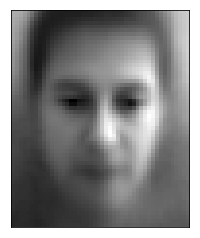
\includegraphics[width=0.6\columnwidth]{Mean_face}
    \caption{Mean face}
    \label{fig:mean face}
\end{figure}
\\We subtracted the mean face to each test image $\phi_n=x_n-\overline{x}$ and formed a matrix $A=[\phi_1,\phi_2,\ldots,\phi_N]\in R^{D\times N}$. We used the function numpy.linalg.eigh to calculate the normalized eigenvectors and eigenvalues in ascending order of the covariance matrix:
\begin{equation}
    S = \frac{1}{N}AA^T \in R^{D\times D}
\end{equation}
\\415 eigenvalues had a values bigger than 70, the remaining had value smaller than $10^{-10}$. The number of non-zero eigenvalues coincides with the rank of the covariance matrix.
\begin{figure}[h]
    \centering
    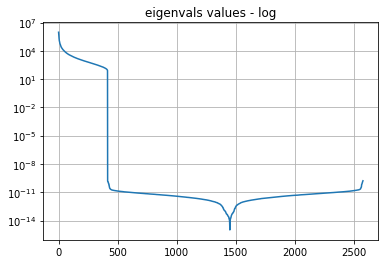
\includegraphics[width=\columnwidth]{images/Eigenvalues_log.png} 
    \caption{semi logarithmic graph of eigenvalues values}
    \label{fig:eigenvalues_log}
\end{figure}
\\The eigenvector corresponding to the biggest eigevalues rapresents the biggest variation in the face space.
\begin{figure}[h]
    \centering
    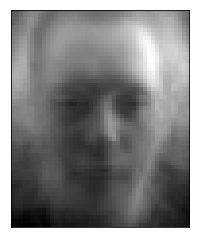
\includegraphics[width=0.3\columnwidth]{images/eigenface001} 
    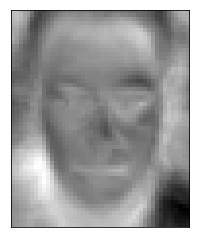
\includegraphics[width=0.3\columnwidth]{images/eigenface010}
    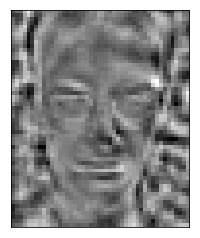
\includegraphics[width=0.3\columnwidth]{images/eigenface100}
    
    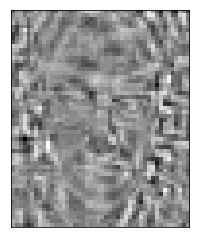
\includegraphics[width=0.3\columnwidth]{images/eigenface200}
    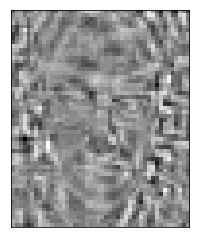
\includegraphics[width=0.3\columnwidth]{images/eigenface200}
    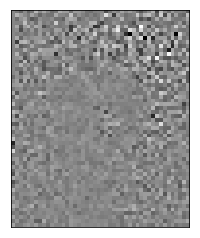
\includegraphics[width=0.3\columnwidth]{images/eigenface500}
    \caption{Eigenfaces of 1,10,100,200,300 and 500 eigenvector}
    \label{fig:eigenfaces}
\end{figure}
The first two eigenfaces capture different facial feature while the ones with a a lower eigevalues capture the frequency, the $500^{th}$  eigenface represents a zero eigenvalue and therefore is just noise. To have the highest accuracy for face recognition we should use 415 eigenvectors (all the non-zero ones) but we could get a good accuracy even with less, we will see the difference in accuracy in \textbf{1.4}. If we devide the eigenvalues vector by the sum of the eigenvalues vector we can see that the first 4 values account for $49.1\%$ of the variance and the last 4 non-zero values account for $85\times 10^{-3}\%$ of the variance.
\begin{table}[h]
    \centering
    \begin{tabular}{|c|c|c|c|}
        \hline
        0.209976    & 0.113739   & 0.107269    & 0.0599219   \\ \hline
        2.1759e-05 & 2.042e-05 & 2.0203e-05 & 1.7459e-05 \\ \hline
    \end{tabular}
    \vspace{2.00mm}
    \caption{Top row: first 4 values of eigenvalues/sum(eigenvalues). Bottom row: last 4 non-zero eigenvalues of eigenvalues/sum(eigenvalues}
    \label{tab:eigenfacesvalue}
\end{table}

\subsection{Eigenfaces - b}

We used the function numpy.linalg.eigh to calculate the normalized eigenvectors and eigenvalues in ascending order of the covariance matrix:
\begin{equation}
    S = \frac{1}{N}A^TA \in R^{N\times N}
\end{equation}
The low dimensional eigenvectors matrix is a $416\times 416$ square matrix while the low dimensional eigenvalues vector has a length of $416$. The first $415$ ($N-1$) eigenvalues are non-zero and they are equal to the first 415 high dimensional eigenvalues. The following relations bewteen $u_i$ (high dimensional eigenvector) and $v_i$ (low dimensional eigenvector) holds:
\begin{equation}
    u_i = ||Av_i||
\end{equation}

Low dimensional computation of eigenspace is quicker to compute, it takes $0.05s$ compare to $2.32s$ for the high dimensional but it requires an extra step to be used for face recognition.


\subsection{Application of Eigenfaces - a}
We calculated $a_{ni} = \phi^T_n , i=1,\ldots,M$ for each $u_i$ and collected all the results in one vector $\omega_n = [a_{n1}, a_{n2},\ldots,a_{nM}]^T$ and reconstructed the faces using:
\begin{equation}
    \widetilde{x}_n = \overline{x} + \sum^M_{i=1}a_{ni}u_i
\end{equation}

\begin{figure}[h]
    \centering
    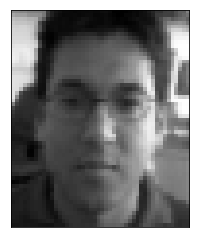
\includegraphics[width=0.3\columnwidth]{images/original_image_213} 
    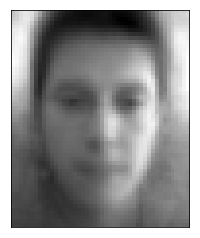
\includegraphics[width=0.3\columnwidth]{images/213_reconstructed_M=10}
    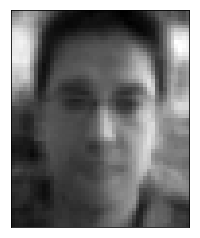
\includegraphics[width=0.3\columnwidth]{images/213_reconstructed_M=50}
    
    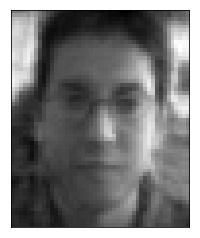
\includegraphics[width=0.3\columnwidth]{images/213_reconstructed_M=100}
    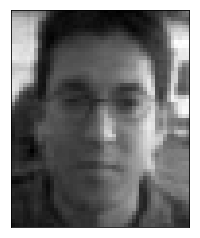
\includegraphics[width=0.3\columnwidth]{images/213_reconstructed_M=200}
    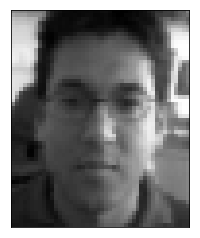
\includegraphics[width=0.3\columnwidth]{images/213_reconstructed_M=415}
    \caption{Original face and reconstructed faces with number of PCA basis = 10, 50, 100, 200, 415.}
    \label{fig:reconstructed faces}
\end{figure}
Increasing the number of PCA bases the quality of the pictures improves, since the first PCA bases have an higher weighting(see previous question), the change from 10 to 100 basis is more noticeable that the change from 100 to 415.

\subsection{Application of Eigenspaces - b}
Perform PCA-based face recognition by the NN classification and alternative method learnt i.e. using the reconstruction errors. Report and discuss, including: recognition accuracies (success rates), example success and failure cases, the confusion matrices,
time/memory, by varying the hyper-parameter values. Give insights and reasons behind your observations. 

The NN classifier has an accuracy of $67.31\%$ and a running time of $0.19s$ while the alternative method classifier has an accuracy of $79.8\%$ and a running time of $2.37$

\begin{table}[h]
\centering
\begin{tabular}{llllllllllllll}
\cellcolor[HTML]{9AFF99}2 & 2                         & 0                         & 0                         & 0                         & 0                         & 0                         & 0                         & 0                         & 0                         & 0                         & 0                         & 1                         & 0                         \\
0                         & \cellcolor[HTML]{9AFF99}0 & 0                         & 0                         & 0                         & 0                         & 0                         & 0                         & 0                         & 0                         & 0                         & 0                         & 0                         & 0                         \\
0                         & 0                         & \cellcolor[HTML]{9AFF99}2 & 0                         & 0                         & 0                         & 0                         & 0                         & 0                         & 0                         & 0                         & 0                         & 0                         & 0                         \\
0                         & 0                         & 0                         & \cellcolor[HTML]{9AFF99}2 & 0                         & 0                         & 0                         & 0                         & 0                         & 0                         & 0                         & 0                         & 0                         & 0                         \\
0                         & 0                         & 0                         & 0                         & \cellcolor[HTML]{9AFF99}2 & 0                         & 0                         & 0                         & 0                         & 0                         & 0                         & 0                         & 0                         & 0                         \\
0                         & 0                         & 0                         & 0                         & 0                         & \cellcolor[HTML]{9AFF99}2 & 0                         & 0                         & 0                         & 0                         & 0                         & 0                         & 0                         & 0                         \\
0                         & 0                         & 0                         & 0                         & 0                         & 0                         & \cellcolor[HTML]{9AFF99}2 & 0                         & 0                         & 0                         & 0                         & 0                         & 0                         & 0                         \\
0                         & 0                         & 0                         & 0                         & 0                         & 0                         & 0                         & \cellcolor[HTML]{9AFF99}2 & 0                         & 0                         & 0                         & 0                         & 0                         & 0                         \\
0                         & 0                         & 0                         & 0                         & 0                         & 0                         & 0                         & 0                         & \cellcolor[HTML]{9AFF99}2 & 0                         & 0                         & 0                         & 0                         & 0                         \\
0                         & 0                         & 0                         & 0                         & 0                         & 0                         & 0                         & 0                         & 0                         & \cellcolor[HTML]{9AFF99}2 & 0                         & 0                         & 0                         & 0                         \\
0                         & 0                         & 0                         & 0                         & 0                         & 0                         & 0                         & 0                         & 0                         & 0                         & \cellcolor[HTML]{9AFF99}2 & 0                         & 0                         & 0                         \\
0                         & 0                         & 0                         & 0                         & 0                         & 0                         & 0                         & 0                         & 0                         & 0                         & 0                         & \cellcolor[HTML]{9AFF99}2 & 0                         & 0                         \\
0                         & 0                         & 0                         & 0                         & 0                         & 0                         & 0                         & 0                         & 0                         & 0                         & 0                         & 0                         & \cellcolor[HTML]{9AFF99}1 & 0                         \\
0                         & 0                         & 0                         & 0                         & 0                         & 0                         & 0                         & 0                         & 0                         & 0                         & 0                         & 0                         & 0                         & \cellcolor[HTML]{9AFF99}2
\end{tabular}
    \caption{Nearest Neighbour confusion matrix for the first 13 classes}
    \label{tab:NN_confusion_matrix}
\end{table}

\begin{table}[h]
\centering
\begin{tabular}{llllllllllllll}
\cellcolor[HTML]{9AFF99}2 & 0                         & 0                         & 0                         & 0                         & 0                         & 0                         & 0                         & 0                         & 0                         & 0                         & 0                         & 1                         & 0                         \\
0                         & \cellcolor[HTML]{9AFF99}2 & 0                         & 0                         & 0                         & 0                         & 0                         & 0                         & 0                         & 0                         & 0                         & 0                         & 0                         & 0                         \\
0                         & 0                         & \cellcolor[HTML]{9AFF99}2 & 0                         & 0                         & 0                         & 0                         & 0                         & 0                         & 0                         & 0                         & 0                         & 0                         & 0                         \\
0                         & 0                         & 0                         & \cellcolor[HTML]{9AFF99}2 & 0                         & 0                         & 0                         & 0                         & 0                         & 0                         & 0                         & 0                         & 0                         & 0                         \\
0                         & 0                         & 0                         & 0                         & \cellcolor[HTML]{9AFF99}2 & 0                         & 0                         & 0                         & 0                         & 0                         & 0                         & 0                         & 0                         & 0                         \\
0                         & 0                         & 0                         & 0                         & 0                         & \cellcolor[HTML]{9AFF99}2 & 0                         & 0                         & 0                         & 0                         & 0                         & 0                         & 0                         & 0                         \\
0                         & 0                         & 0                         & 0                         & 0                         & 0                         & \cellcolor[HTML]{9AFF99}2 & 0                         & 0                         & 0                         & 0                         & 0                         & 0                         & 0                         \\
0                         & 0                         & 0                         & 0                         & 0                         & 0                         & 0                         & \cellcolor[HTML]{9AFF99}2 & 0                         & 0                         & 0                         & 0                         & 0                         & 0                         \\
0                         & 0                         & 0                         & 0                         & 0                         & 0                         & 0                         & 0                         & \cellcolor[HTML]{9AFF99}2 & 0                         & 0                         & 0                         & 0                         & 0                         \\
0                         & 0                         & 0                         & 0                         & 0                         & 0                         & 0                         & 0                         & 0                         & \cellcolor[HTML]{9AFF99}2 & 0                         & 0                         & 0                         & 0                         \\
0                         & 0                         & 0                         & 0                         & 0                         & 0                         & 0                         & 0                         & 0                         & 0                         & \cellcolor[HTML]{9AFF99}2 & 0                         & 0                         & 0                         \\
0                         & 0                         & 0                         & 0                         & 0                         & 0                         & 0                         & 0                         & 0                         & 0                         & 0                         & \cellcolor[HTML]{9AFF99}2 & 0                         & 0                         \\
0                         & 0                         & 0                         & 0                         & 0                         & 0                         & 0                         & 0                         & 0                         & 0                         & 0                         & 0                         & \cellcolor[HTML]{9AFF99}1 & 0                         \\
0                         & 0                         & 0                         & 0                         & 0                         & 0                         & 0                         & 0                         & 0                         & 0                         & 0                         & 0                         & 0                         & \cellcolor[HTML]{9AFF99}2
\end{tabular}
    \caption{Alternative method confusion matrix for the first 13 classes}
    \label{tab:AM_confusion_matrix}
\end{table}

\section{Q2}

PCA is a generative model which projects data onto an eigenface subspace to maximize the variance of the data set. This is described by the following objective function: 

\begin{equation}
	J = u^TSu
\end{equation}
\\LDA is a discriminative model which aims to maximize the ratio between the between-class and within-class data scatter, described in the function below: 
\begin{equation}
	J(w) = \frac{w^TS_bw}{w^TS_ww}
\end{equation}
\\To develop a subspace for each individual approach, we represent the problem as a Lagrange multiplier formulation, and solve to yield a generalized eigenvalue-eigenvector result. The Lagrangian formulation of the PCA and LDA optimization problems are given below:
\begin{equation}
 
	L_{PCA}=u^TSu +\lambda (1-u^Tt)
	L_{LDA} = w^TS_Bw+\lambda (k-w^TSww)
\end{equation}
\\To obtain a hybrid subspace which simultaneously extracts generative and discriminative features, we must formulate an optimization problem involving both functions above.
\begin{equation}
L=L_{PCA} + L_{LDA}
\end{equation}

Note that we will represent u and w by a new variable v, since they now refer to the same subspace. 
\begin{equation}
	L=v^TSv+\lambda (1-v^Tv)+v^TS_Bv+\lambda (k-v^TS_wv)=v^TSv+v^TS_Bv+\lambda (1+k-v^Tv-v^TS_wv)
\end{equation}
Setting the gradient, with respect to v, to zero:
\begin{equation}
	\frac{dL}{dv} = Sv-\lambda v+2(S_B-\lambda S_w)v=0
	\frac{dL}{dv}=(v^TS^T)+(v^TS^T_B)-\lambda (2v+(v^TS^T_w+v^TS_w))=0
\end{equation}
\\This can be simplified using the property for symmetric matrices and the quadratic matrix derivative relation, shown below, respectively:
\begin{equation}
	S^T=S
	\frac{\partial x^TAx}{\partial x} = x^T(A^T+A) = x^TA^T+x^TA
\end{equation}
Which yields:
\begin{equation}
	\frac{dL}{dV} =2Sv+2S_Bv-2\lambda S_wv-2\lambdav=0
	Sv+S_Bv+\lambda S_wv-\lambda v=0
	\lambda (S_w-I)v=(S+S_B)v
	\lambda v=(S+S_B)(S_w-I)^{-1}v
\end{equation}
Therefore, by solving this eigenvalue-eigenvector equation and isolating the most significant eigenvectors, we could produce a subspace which describes a combination of generative and discriminative features. 

Note that the equations detailed were derived using the provided lecture notes. 


\section{Q3}

\subsection{PCA-LDA}
While PCA projections allow for image reconstruction from a low dimensional basis, LDA is a necessary extension for class discrimination . Subjecting a data set to both methods in succession, followed by NN classification, can combine the benefits of dimensional reduction and class separation from the eigenface space and Fischer space, respectively. 

The LDA method involves optimizing parameter W such that the ratio of the determinant of the between-class scatter matrix ($S_B$) and that of the within-class scatter matrix ($S_W$) is maximized, described by the equation:

\begin{equation}
	W_{opt} = argmax_w \frac{|W^TS_BW|}{W^TS_WW}=[w_1,w_2,\ldots,w_{M_{LDA}}]
\end{equation} 

The matrices involved are defined as:
\begin{equation}
	S_B=\sum ^c_{i=1}(m_i-m)(m_i-m)^T
	S_w=\sum ^c_{i=1} \sum _{c \in C_i} (x-m_i)(x-m_i)^T
\end{equation}
Where \textbf{$m_i$} is the class mean,\textbf{m} is the global mean, and \textbf{x} is the input image data. 

To obtain the set of generalized eigenvectors, \textbf{$w_i$}, we collate the eigenvectors corresponding to the $M_LDA$ largest eigenvalues obtained from the following relation:
\begin{equation}
	S_Bw_i=\lambda _iS_Ww_i,	i=1,\ldots,M_{LDA}
\end{equation} 
Given the existing definitions of the scatter matrices, the rank of $S_W\in \Re ^{n\times n}$ has an upper limit of N-c, however the number of images, N, is far lower than the number of pixels per image, n, rendering the matrix singular and the above equation unsolvable. 

To solve this, we first conduct PCA and apply LDA to the resulting, low-dimensional eigenface space projected data, represented by ω. This adjusts the $S_W$ matrix as follows:
\begin{equation}
		S_w=\sum ^c_{i=1} \sum _{c \in C_i} (\omega_c_i-m_i)(\omega_c_i-m_i)^T
\end{equation}
Giving it the dimensions ($M_{PCA}$, $M_{PCA}$).
While $M_{PCA}$ is bounded by the rank of $S_W$, N-c, $M_{LDA}$ is limited by the rank of $S_B$, $c-1$. The plot below shows the effect of varying $M_{PCA}$ and $M_{LDA}$ on recognition accuracy. 

\begin{figure}[h]
    \centering
    \includegraphics[width=\columnwidth]{images/confusio_matrix_Q3} 
    \caption{Accuracy with respect to parameters $M_{PCA}$ and $M_{LDA}$
    \label{fig:accuracy_Q3}
\end{figure}
From this plot we can see that, in general, increasing both $M_{PCA}$ and $M_{LDA}$ increases the accuracy of the classifier. However, when looking at the plots corresponding to the two highest values of $M_{PCA}$, specifically together with low $M_{LDA}$ values, the accuracy suffers. This depicts how high dimensionality in feature space can lead to loss of generality and thus robustness of the classifier. The overall plot also clearly demonstrates the importance of high $M_{LDA}$ in class separation. 

Recognition accuracy can be depicted by the confusion matrix, shown below for $M_{PCA}=200$ and $M_{LDA}=50$. The ideal scenario would be depicted exclusively by a black diagonal line, indicating two correct predictions, for both testing images in each class. 
\begin{figure}[h]
    \centering
    \includegraphics[width=\columnwidth]{images/confusio_matrix_Q3} 
    \caption{confusion matrix}   \label{fig:confusion_Q3}
\end{figure}
The confusion matrix can be used to see where data is being misclassified. For example, the image truly labelled as class 48 is wrongly classified both times as label 29. This implies that these images have similar features, which can be confirmed qualitatively in the table below. In cases like these, the images could be further processed for more selective discrimination. 

\begin{figure}[h]
    \centering
    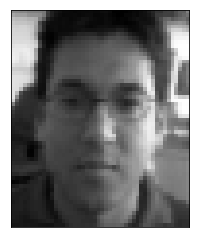
\includegraphics[width=0.4\columnwidth]{images/original_image_213} 
    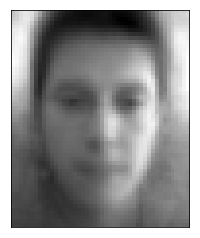
\includegraphics[width=0.4\columnwidth]{images/213_reconstructed_M=10}
    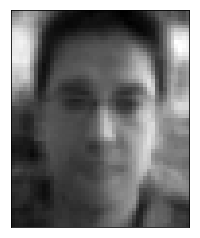
\includegraphics[width=0.4\columnwidth]{images/213_reconstructed_M=50}
    
    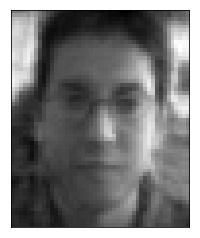
\includegraphics[width=0.4\columnwidth]{images/213_reconstructed_M=100}

    \caption{Left column are true, right column are predicted}
    \label{fig:predicted_faces}
\end{figure}

\subsection{PCA-LDA Ensemble}
High dimensionality in the Fischer space leads to overfitting. To compromise between generality and discriminative ability, we develop multiple low dimensional classifiers with either randomly sampled features or randomly sampled training samples and combine their outputs to increase confidence in the results. 

To produce classifiers using randomly sampled features, we sample $M_{PCA}=M_0+M_1$ of the $N_{train}-1$ number of eigenfaces with non-zero eigenvalues. $M_0$ refers to a fixed set of the largest eigenfaces, while $M_1$ refers to a set randomly sampled from the remaining $N_{train}-1-M_0$ eigenfaces. By conducting this $K_1$ times, we develop $K_1$ random subspaces. 
\begin{figure}[h]
    \centering
    \includegraphics[width=\columnwidth]{images/confusio_matrix_Q3} 
    \caption{Accuracy with respect to parameters $M_0, M_1$ and $K$}   \end{figure}
    
The graph above reveals the general trend that the higher value of $M_0$, the greater the accuracy of the model. This is justifiable since $M_0$ retains the most significant structural information of the image, which is why it remains fixed in the during the randomization process. 

Random sampling of training data, known as “bagging”, produces samples of the given training set. The procedure involves randomly selecting $L_1$ classes. Note that only the classes are sampled, rather than the data itself. Conducting this $K_2$ times develops $K_2$ random subspaces. 
\begin{figure}[h]
    \centering
    \includegraphics[width=\columnwidth]{images/confusio_matrix_Q3} 
    \caption{Accuracy with respect to parameters $L_1$ and $K$}  
\end{figure}  
In theory, the higher the values of $K_1$ and $K_2$, the more likely that the combination of these classifiers cover all features and classes, leading to higher accuracy. Expressed differently, the error of the “committee” of subspaces should be lower than that of an individual model by the relation}
\begin{equation}
	E_{committee}=\frac{1}{T} E_{individual}
\end{equation}  

The results do not show this, suggesting that the already high number of samples within each class provides enough variation so that randomization does not improve discrimination. 

The fusion technique used was majority voting, where the most frequently appearing prediction over every subspace is assigned to the test image. Other techniques which could be employed to improve accuracy include using a set of nearest neighbors to develop a probability distribution for the assigned label. For a set of K subspaces, the distributions for each subspace can be combined through summation or multiplication to exaggerate the most likely label. 

%------------------------------------------------------------------------
\section{Formatting your paper}

All text must be in a two-column format. The total allowable width of the
text area is $6\frac78$ inches (17.5 cm) wide by $8\frac78$ inches (22.54
cm) high. Columns are to be $3\frac14$ inches (8.25 cm) wide, with a
$\frac{5}{16}$ inch (0.8 cm) space between them. The main title (on the
first page) should begin 1.0 inch (2.54 cm) from the top edge of the
page. The second and following pages should begin 1.0 inch (2.54 cm) from
the top edge. On all pages, the bottom margin should be 1-1/8 inches (2.86
cm) from the bottom edge of the page for $8.5 \times 11$-inch paper; for A4
paper, approximately 1-5/8 inches (4.13 cm) from the bottom edge of the
page.

%-------------------------------------------------------------------------
\subsection{Margins and page numbering}

All printed material, including text, illustrations, and charts, must be kept
within a print area 6-7/8 inches (17.5 cm) wide by 8-7/8 inches (22.54 cm)
high.
Page numbers should be in footer with page numbers, centered and .75
inches from the bottom of the page and make it start at the correct page
number rather than the 4321 in the example.  To do this fine the line (around
line 23)
\begin{verbatim}
%\ifcvprfinal\pagestyle{empty}\fi
\setcounter{page}{4321}
\end{verbatim}
where the number 4321 is your assigned starting page.

Make sure the first page is numbered by commenting out the first page being
empty on line 46
\begin{verbatim}
%\thispagestyle{empty}
\end{verbatim}


%-------------------------------------------------------------------------
\subsection{Type-style and fonts}

Wherever Times is specified, Times Roman may also be used. If neither is
available on your word processor, please use the font closest in
appearance to Times to which you have access.

MAIN TITLE. Center the title 1-3/8 inches (3.49 cm) from the top edge of
the first page. The title should be in Times 14-point, boldface type.
Capitalize the first letter of nouns, pronouns, verbs, adjectives, and
adverbs; do not capitalize articles, coordinate conjunctions, or
prepositions (unless the title begins with such a word). Leave two blank
lines after the title.

AUTHOR NAME(s) and AFFILIATION(s) are to be centered beneath the title
and printed in Times 12-point, non-boldface type. This information is to
be followed by two blank lines.

The ABSTRACT and MAIN TEXT are to be in a two-column format.

MAIN TEXT. Type main text in 10-point Times, single-spaced. Do NOT use
double-spacing. All paragraphs should be indented 1 pica (approx. 1/6
inch or 0.422 cm). Make sure your text is fully justified---that is,
flush left and flush right. Please do not place any additional blank
lines between paragraphs.

Figure and table captions should be 9-point Roman type as in
Figures~\ref{fig:onecol} and~\ref{fig:short}.  Short captions should be centred.

\noindent Callouts should be 9-point Helvetica, non-boldface type.
Initially capitalize only the first word of section titles and first-,
second-, and third-order headings.

FIRST-ORDER HEADINGS. (For example, {\large \bf 1. Introduction})
should be Times 12-point boldface, initially capitalized, flush left,
with one blank line before, and one blank line after.

SECOND-ORDER HEADINGS. (For example, { \bf 1.1. Database elements})
should be Times 11-point boldface, initially capitalized, flush left,
with one blank line before, and one after. If you require a third-order
heading (we discourage it), use 10-point Times, boldface, initially
capitalized, flush left, preceded by one blank line, followed by a period
and your text on the same line.

%-------------------------------------------------------------------------
\subsection{Footnotes}

Please use footnotes\footnote {This is what a footnote looks like.  It
often distracts the reader from the main flow of the argument.} sparingly.
Indeed, try to avoid footnotes altogether and include necessary peripheral
observations in
the text (within parentheses, if you prefer, as in this sentence).  If you
wish to use a footnote, place it at the bottom of the column on the page on
which it is referenced. Use Times 8-point type, single-spaced.


%-------------------------------------------------------------------------
\subsection{References}

List and number all bibliographical references in 9-point Times,
single-spaced, at the end of your paper. When referenced in the text,
enclose the citation number in square brackets, for
example~\cite{Authors14}.  Where appropriate, include the name(s) of
editors of referenced books.

\begin{table}
\begin{center}
\begin{tabular}{|l|c|}
\hline
Method & Frobnability \\
\hline\hline
Theirs & Frumpy \\
Yours & Frobbly \\
Ours & Makes one's heart Frob\\
\hline
\end{tabular}
\end{center}
\caption{Results.   Ours is better.}
\end{table}

%-------------------------------------------------------------------------
\subsection{Illustrations, graphs, and photographs}

All graphics should be centered.  Please ensure that any point you wish to
make is resolvable in a printed copy of the paper.  Resize fonts in figures
to match the font in the body text, and choose line widths which render
effectively in print.  Many readers (and reviewers), even of an electronic
copy, will choose to print your paper in order to read it.  You cannot
insist that they do otherwise, and therefore must not assume that they can
zoom in to see tiny details on a graphic.

When placing figures in \LaTeX, it's almost always best to use
\verb+\includegraphics+, and to specify the  figure width as a multiple of
the line width as in the example below
{\small\begin{verbatim}
   \usepackage[dvips]{graphicx} ...
   \includegraphics[width=0.8\linewidth]
                   {myfile.eps}
\end{verbatim}
}


%-------------------------------------------------------------------------
\subsection{Color}

Please refer to the author guidelines on the CVPR 2016 web page for a discussion
of the use of color in your document.

%------------------------------------------------------------------------
\section{Final copy}

You must include your signed IEEE copyright release form when you submit
your finished paper. We MUST have this form before your paper can be
published in the proceedings.


{\small
\bibliographystyle{ieee}
\bibliography{egbib}
}

\end{document}
